\section{ProtoDUNE-ND}
\label{sec:protodune-nd}
In this section, the technical design of the proposed ProtoDUNE-ND at Fermilab is described. First, a consideration of the available neutrino beamlines at Fermilab is carried out in Section~\ref{sec:neutrino-flux}, which shows that the on-axis medium-energy NuMI beam provides a rate closest to that of the future, intense, LBNF beamline~\cite{DUNE3, dune_opt_flux}, making the MINOS hall the ideal location for this prototype. Second, a discussion of the MINOS near detector hall is provided in Section~\ref{sec:minos-hall}, with consideration given to the existing and required infrastructure to support the ProtoDUNE-ND detectors. Then, a discussion of the technical aspects of the ProtoDUNE-ND detector design is given: a description of the ArgonCube 2x2 Demonstrator module is given in Section~\ref{sec:2x2-design}, and a description of potential downstream tracking detectors is given in Section~\ref{sec:tracking_detectors}. %\todo{Modify as appropriate... if there's only ArgonCube information available, we can note the possibility of others being included, and comment on the branch points when decisions about whether to include them or not must be made.}

\subsection{Neutrino flux study}
\label{sec:neutrino-flux}
The LBNF beamline is an intense source of muon (anti-)neutrinos, with a much higher flux of neutrinos than accelerator neutrino beams currently in operation~\cite{DUNE3,dune_opt_flux}. A key design requirement for the DUNE near detectors, and one of the primary concerns motivating this ProtoDUNE-ND proposal, is how well the near detector components will perform in a high multiplicity environment. It is therefore worth asking how suitable existing beamlines are for providing a useful neutrino beam test for the proposed near detector components.

\begin{figure}[htb]
  \centering
  \subfloat[Flux\label{subfig:flux}]    {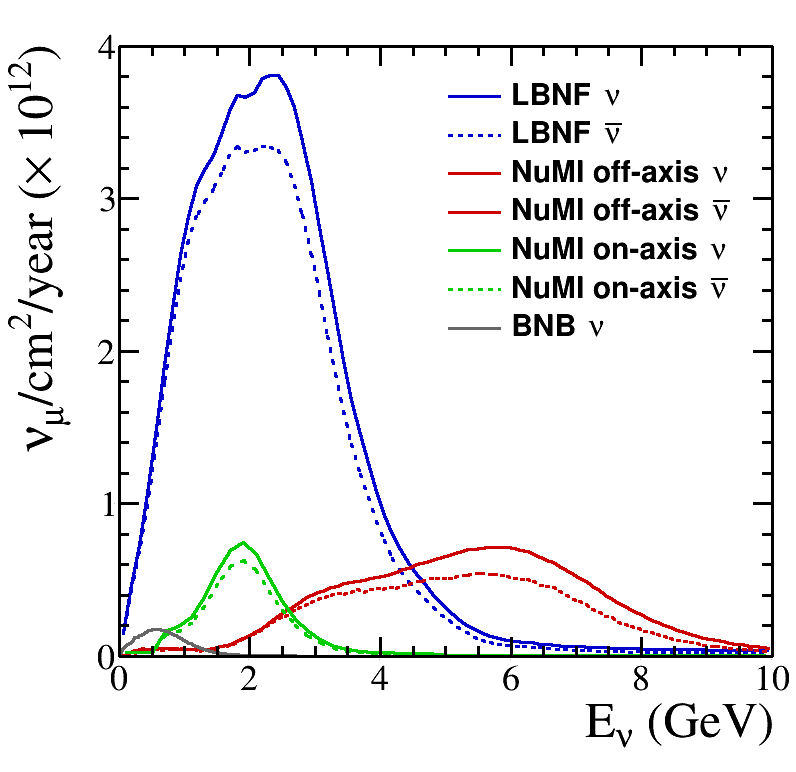
\includegraphics[width=0.5\textwidth]{plots/fnal_flux_comparison.png}}
  \subfloat[Rate\label{subfig:rate}]    {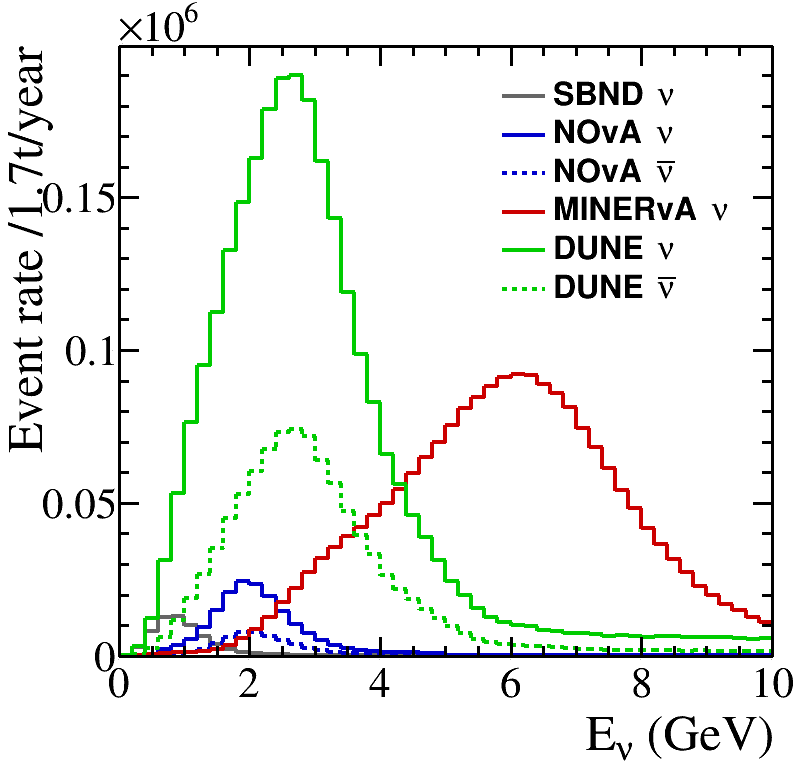
\includegraphics[width=0.5\textwidth]{plots/2x2_Enu_all.png}}
  \caption{Comparison of the absolutely normalized fluxes for different neutrino beamlines at Fermilab, and the expected yearly rates in the ArgonCube 2x2 Demonstrator module's 1.7t active LAr volume as a function of \enu, produced using GENIE v2.12.10 with the ``ValenciaQEBergerSehgalCOHRES'' configuration~\cite{genie}.}
  \label{fig:beam_options}
\end{figure}
In Figure~\ref{subfig:flux}, the currently available neutrino fluxes at various near detector halls in Fermilab are compared, on an absolutely normalized scale, to the LBNF three-horn optimized flux at the 574~m near detector site~\cite{dune_opt_flux}. The currently available neutrino fluxes considered are the on- and 14 mrad. off-axis medium-energy neutrinos from the main injector (NuMI) beam~\cite{numi}, which corresponds to the MINOS and NOvA near detector halls; and the booster neutrino beam (BNB) at the SBND hall~\cite{Antonello:2015lea}. The FY2017 delivered POT was used to produce a yearly flux and rate for the BNB and NuMI beams~\cite{fnal_beam_2017}. It is clear that the proposed LBNF flux is significantly more intense than the fluxes sampled at any existing experimental hall. However, due to the roughly linear relationship between neutrino energy and cross section, the measured rate from the on-axis NuMI beam in the MINOS-ND hall is approximately the same as for the planned LBNF flux, and is therefore the most desirable currently functional experimental hall at Fermilab for a ProtoDUNE-ND test. The rate has been produced with the GENIE neutrino interaction Monte Carlo package~\cite{genie}, using v2.12.10 with the ValenciaQEBergerSehgalCOHRES configuration. Note that the rate is normalized to the active volume of the ArgonCube 2x2 Demonstrator module, showing that significant statistics will be accumulated in a matter of months of ProtoDUNE-ND operation.

\FloatBarrier
\subsection{MINOS near detector hall}
\label{sec:minos-hall}
\begin{itemize}
\item Size of the hall
\item Existing infrastructure required for the test
\item Need to consider whether we need to move anything (e.g. MINERvA) to make space
\item New infrastructure to be put in for the test --> Barry Norris/ Alan Bross. Probably need to discuss language with Steve Brice to make it forceful enough
\end{itemize}

\subsection{ArgonCube 2x2 Demonstrator module}
\label{sec:2x2-design}

ArgonCube, and the Argoncube 2x2 Demonstrator module are described in Ref.~\cite{argoncube_loi}. However, a number of significant changes to the design have been made since then, to account for the advancements made in the ArgonCube R\&D program. In particular, the four modules of the ArgonCube 2x2 Demonstrator module will not test separate technologies, as design choices have already been informed by smaller scale tests. Instead, the modules will be functionally identical, to allow for more sophisticated reconstruction tests.

\begin{figure}[htbp]
\centering
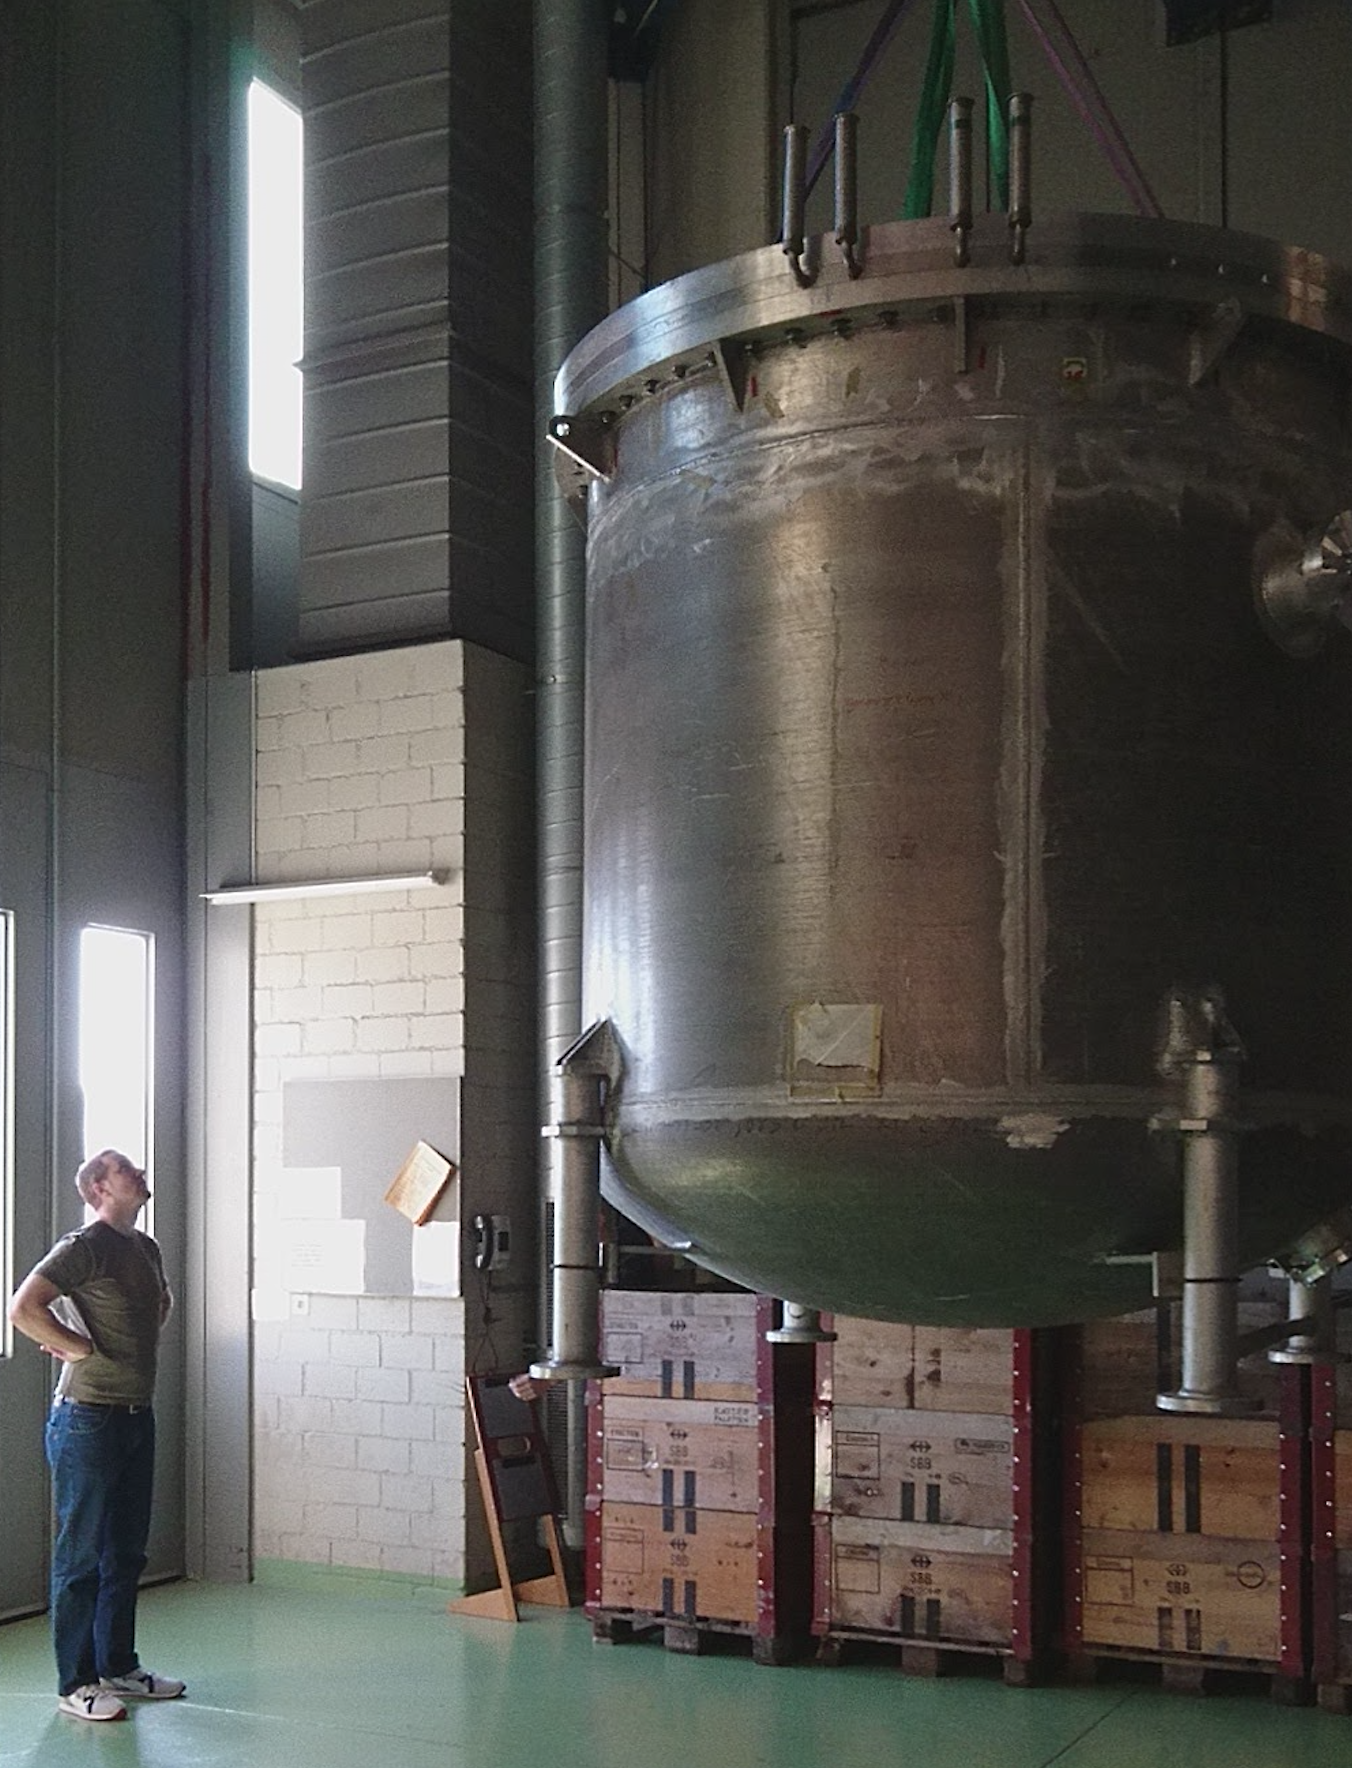
\includegraphics[width=0.45\linewidth]{plots/cryostat.png}
\caption{The liquid nitrogen-cooled and vacuum-insulated cryostat that will host the ArgonCube 2x2 Demonstrator module, reproduced from Ref.~\cite{argoncube_loi}.}
\label{fig:2x2_cryostat}
\end{figure}

The basic principle of ArgonCube is a detector made of self-contained TPC modules sharing a common cryostat. Each module is made of a rectangular box with a square footprint and a height to be optimized in order to meet the physics goals and/or sensitivity constraints. The ArgonCube 2x2 Demonstrator module will be housed within an existing liquid nitrogen (LN2)-cooled and vacuum-insulated cryostat, shown in Figure~\ref{fig:2x2_cryostat}, which is $\sim$\SI{2.2}{\metre} in diameter, and $\sim$\SI{2.8}{\metre} deep, for a total volume of $\sim$\SI{6}{\metre\cubed}. The size of the cryostat sets the dimensions of the modules for the demonstrator. The square base of each module will be \SI{0.67 x 0.67}{\metre}, and the height will be \SI{1.81}{\metre}. This makes the modules comparable in size to, but slightly smaller than, the proposed DUNE near detector, which will have a base of \SI{1 x 1}{\metre}, with a \SI{3.5}{\metre} height; optimized in order to meet the physics goals and sensitivity constraints.

\begin{figure}[htbp]
\centering
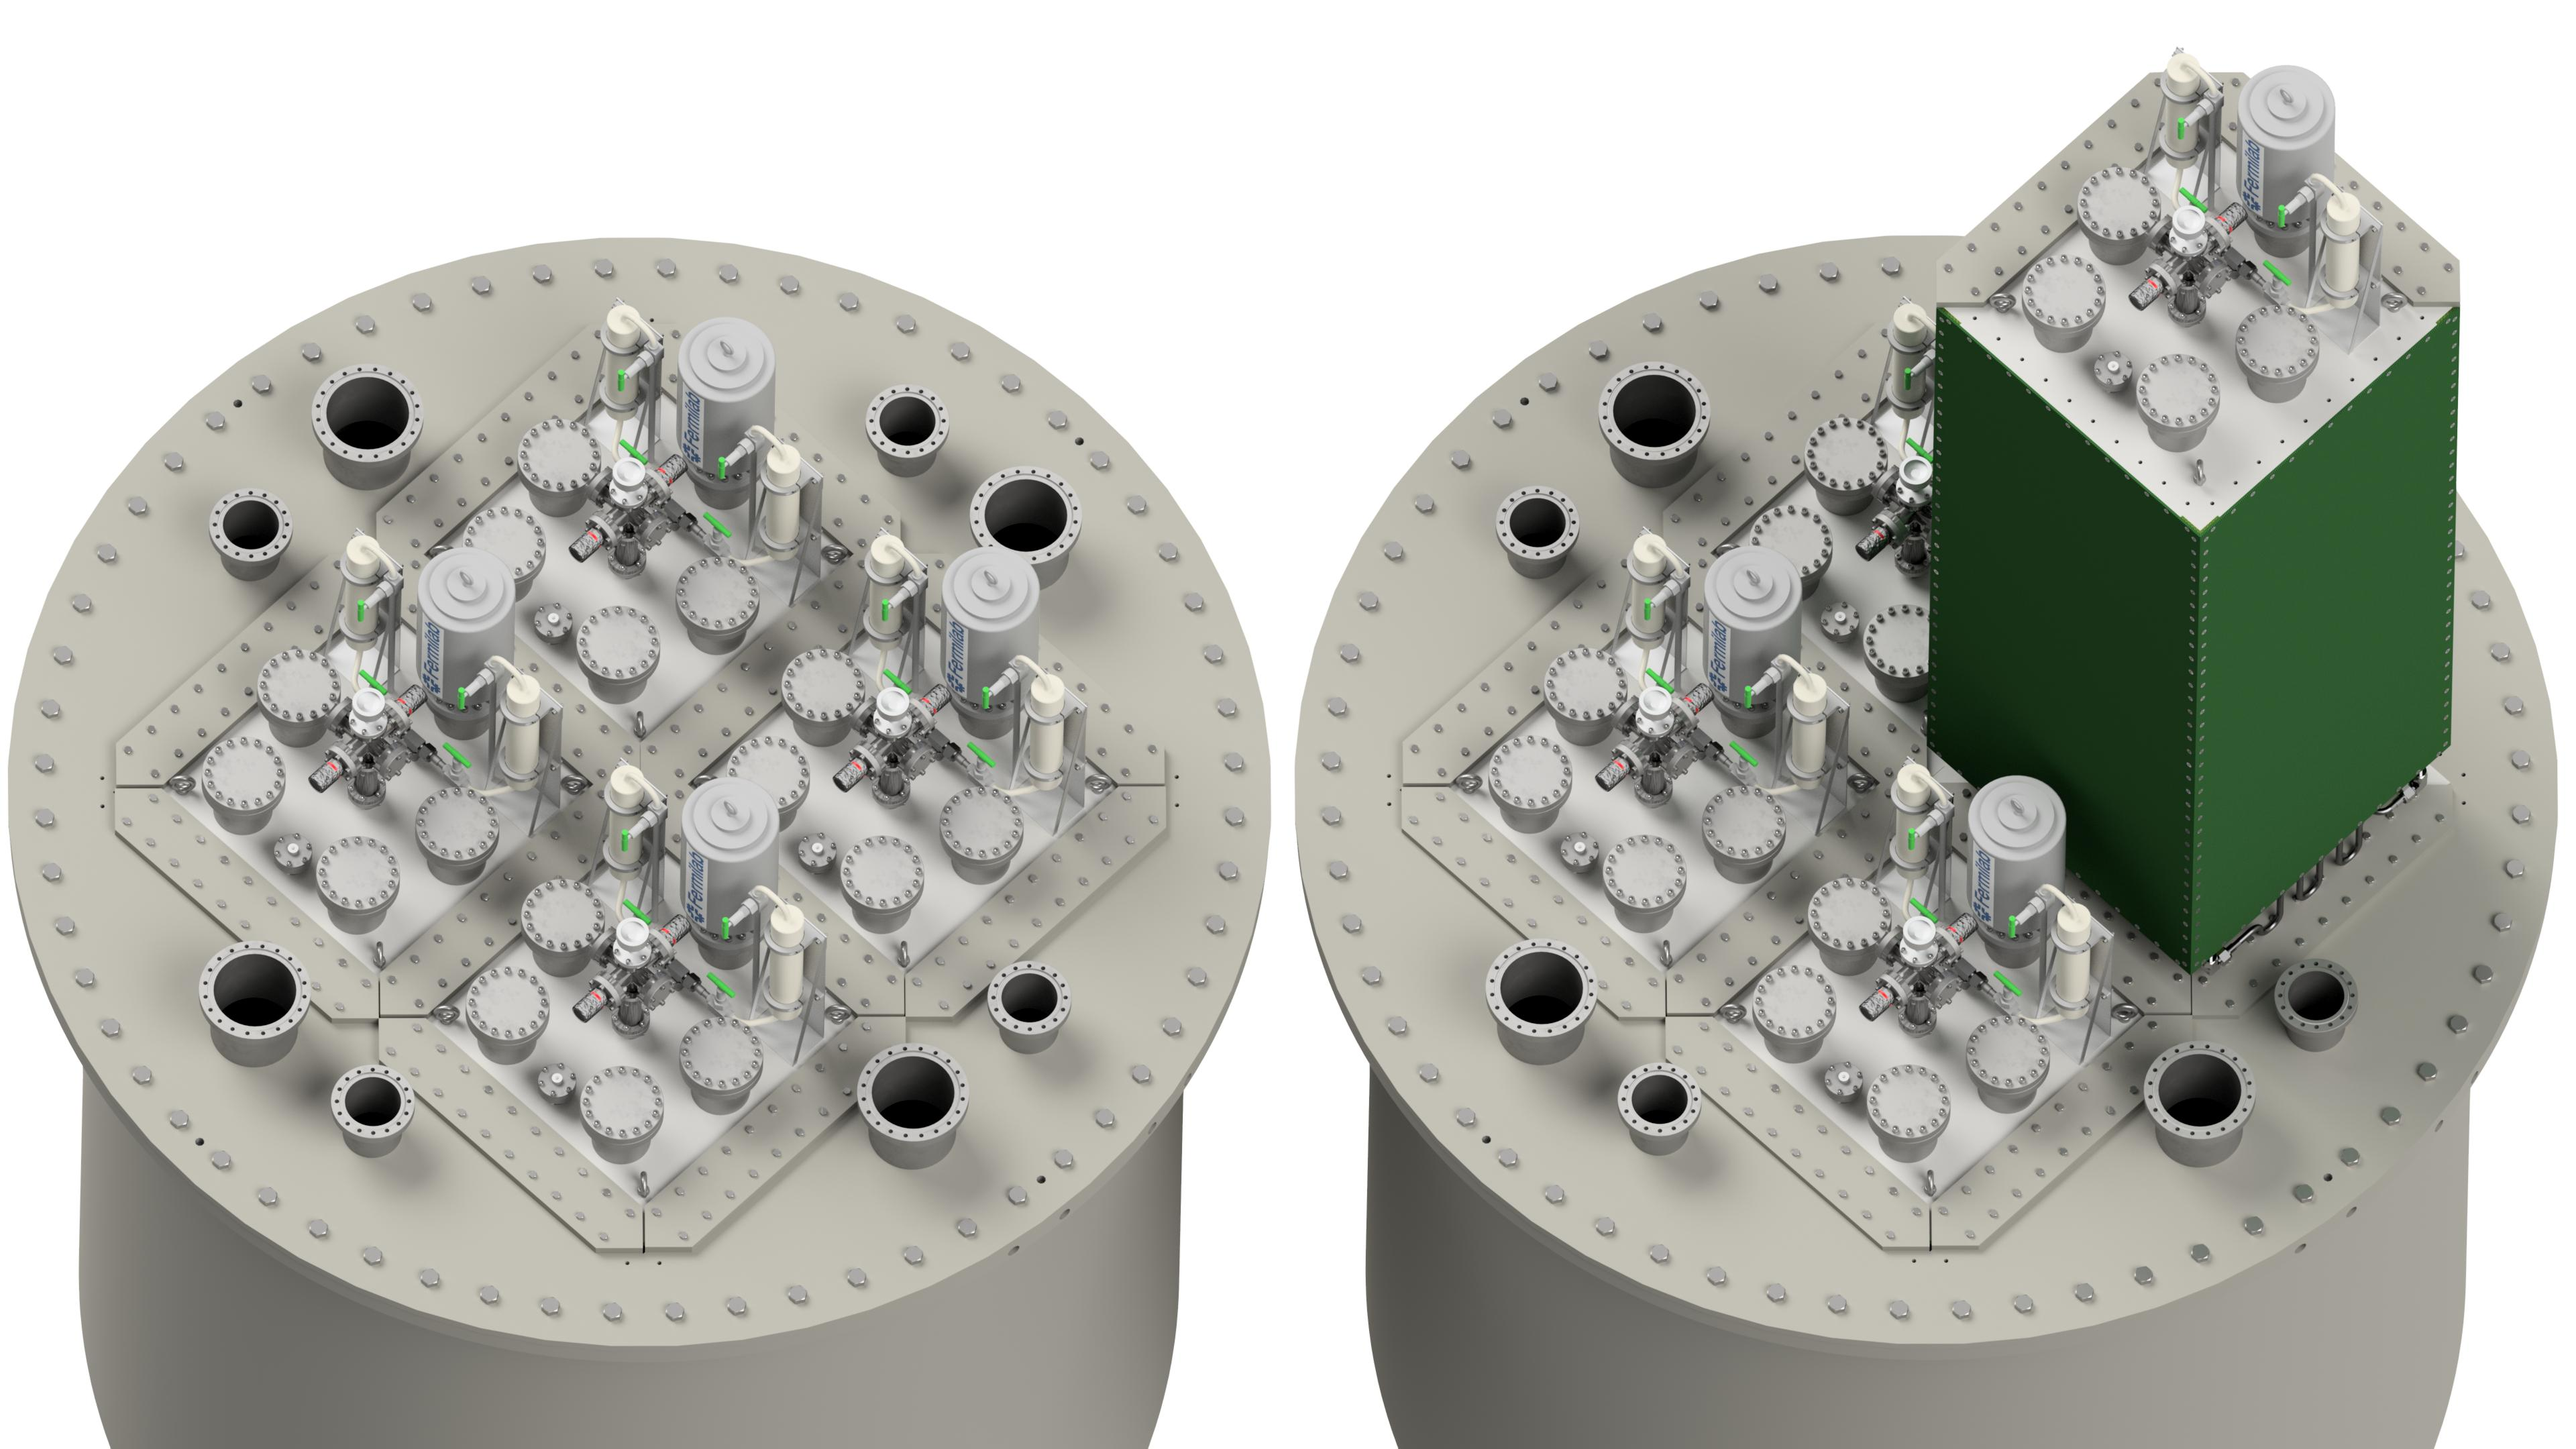
\includegraphics[width=\textwidth]{plots/BathAndModule.png}
\caption{Illustration of the ArgonCube 2x2 Demonstrator module. The four modules are visible, with one of them is partly extracted, on the right. This figure has been reproduced from Ref.~\cite{argoncube_loi}.}
\label{fig:2x2_extraction}
\end{figure}

Individual modules can be extracted or reinserted into a common LAr bath as needed, as is illustrated in Figure~\ref{fig:2x2_extraction}. Pressure inside the modules is kept close to the bath pressure putting almost no hydrostatic force on the module walls, which allows them to be thin, to minimize the inactive material in the walls. The purity of the LAr is maintained within each module independently, as will be described below. As a result, the argon surrounding the modules needs not meet as stringent purity requirements as the argon inside. Under normal operation conditions all modules are inserted with only clearance distances between modules. Cooling power to the bath is supplied by cryocoolers located in unistrumented volumes at the side of the detector called service volumes, and LN2 circulated through lines on the outer surface of the inner cryostat vessel.

\begin{figure}[tbp]
  \centering
  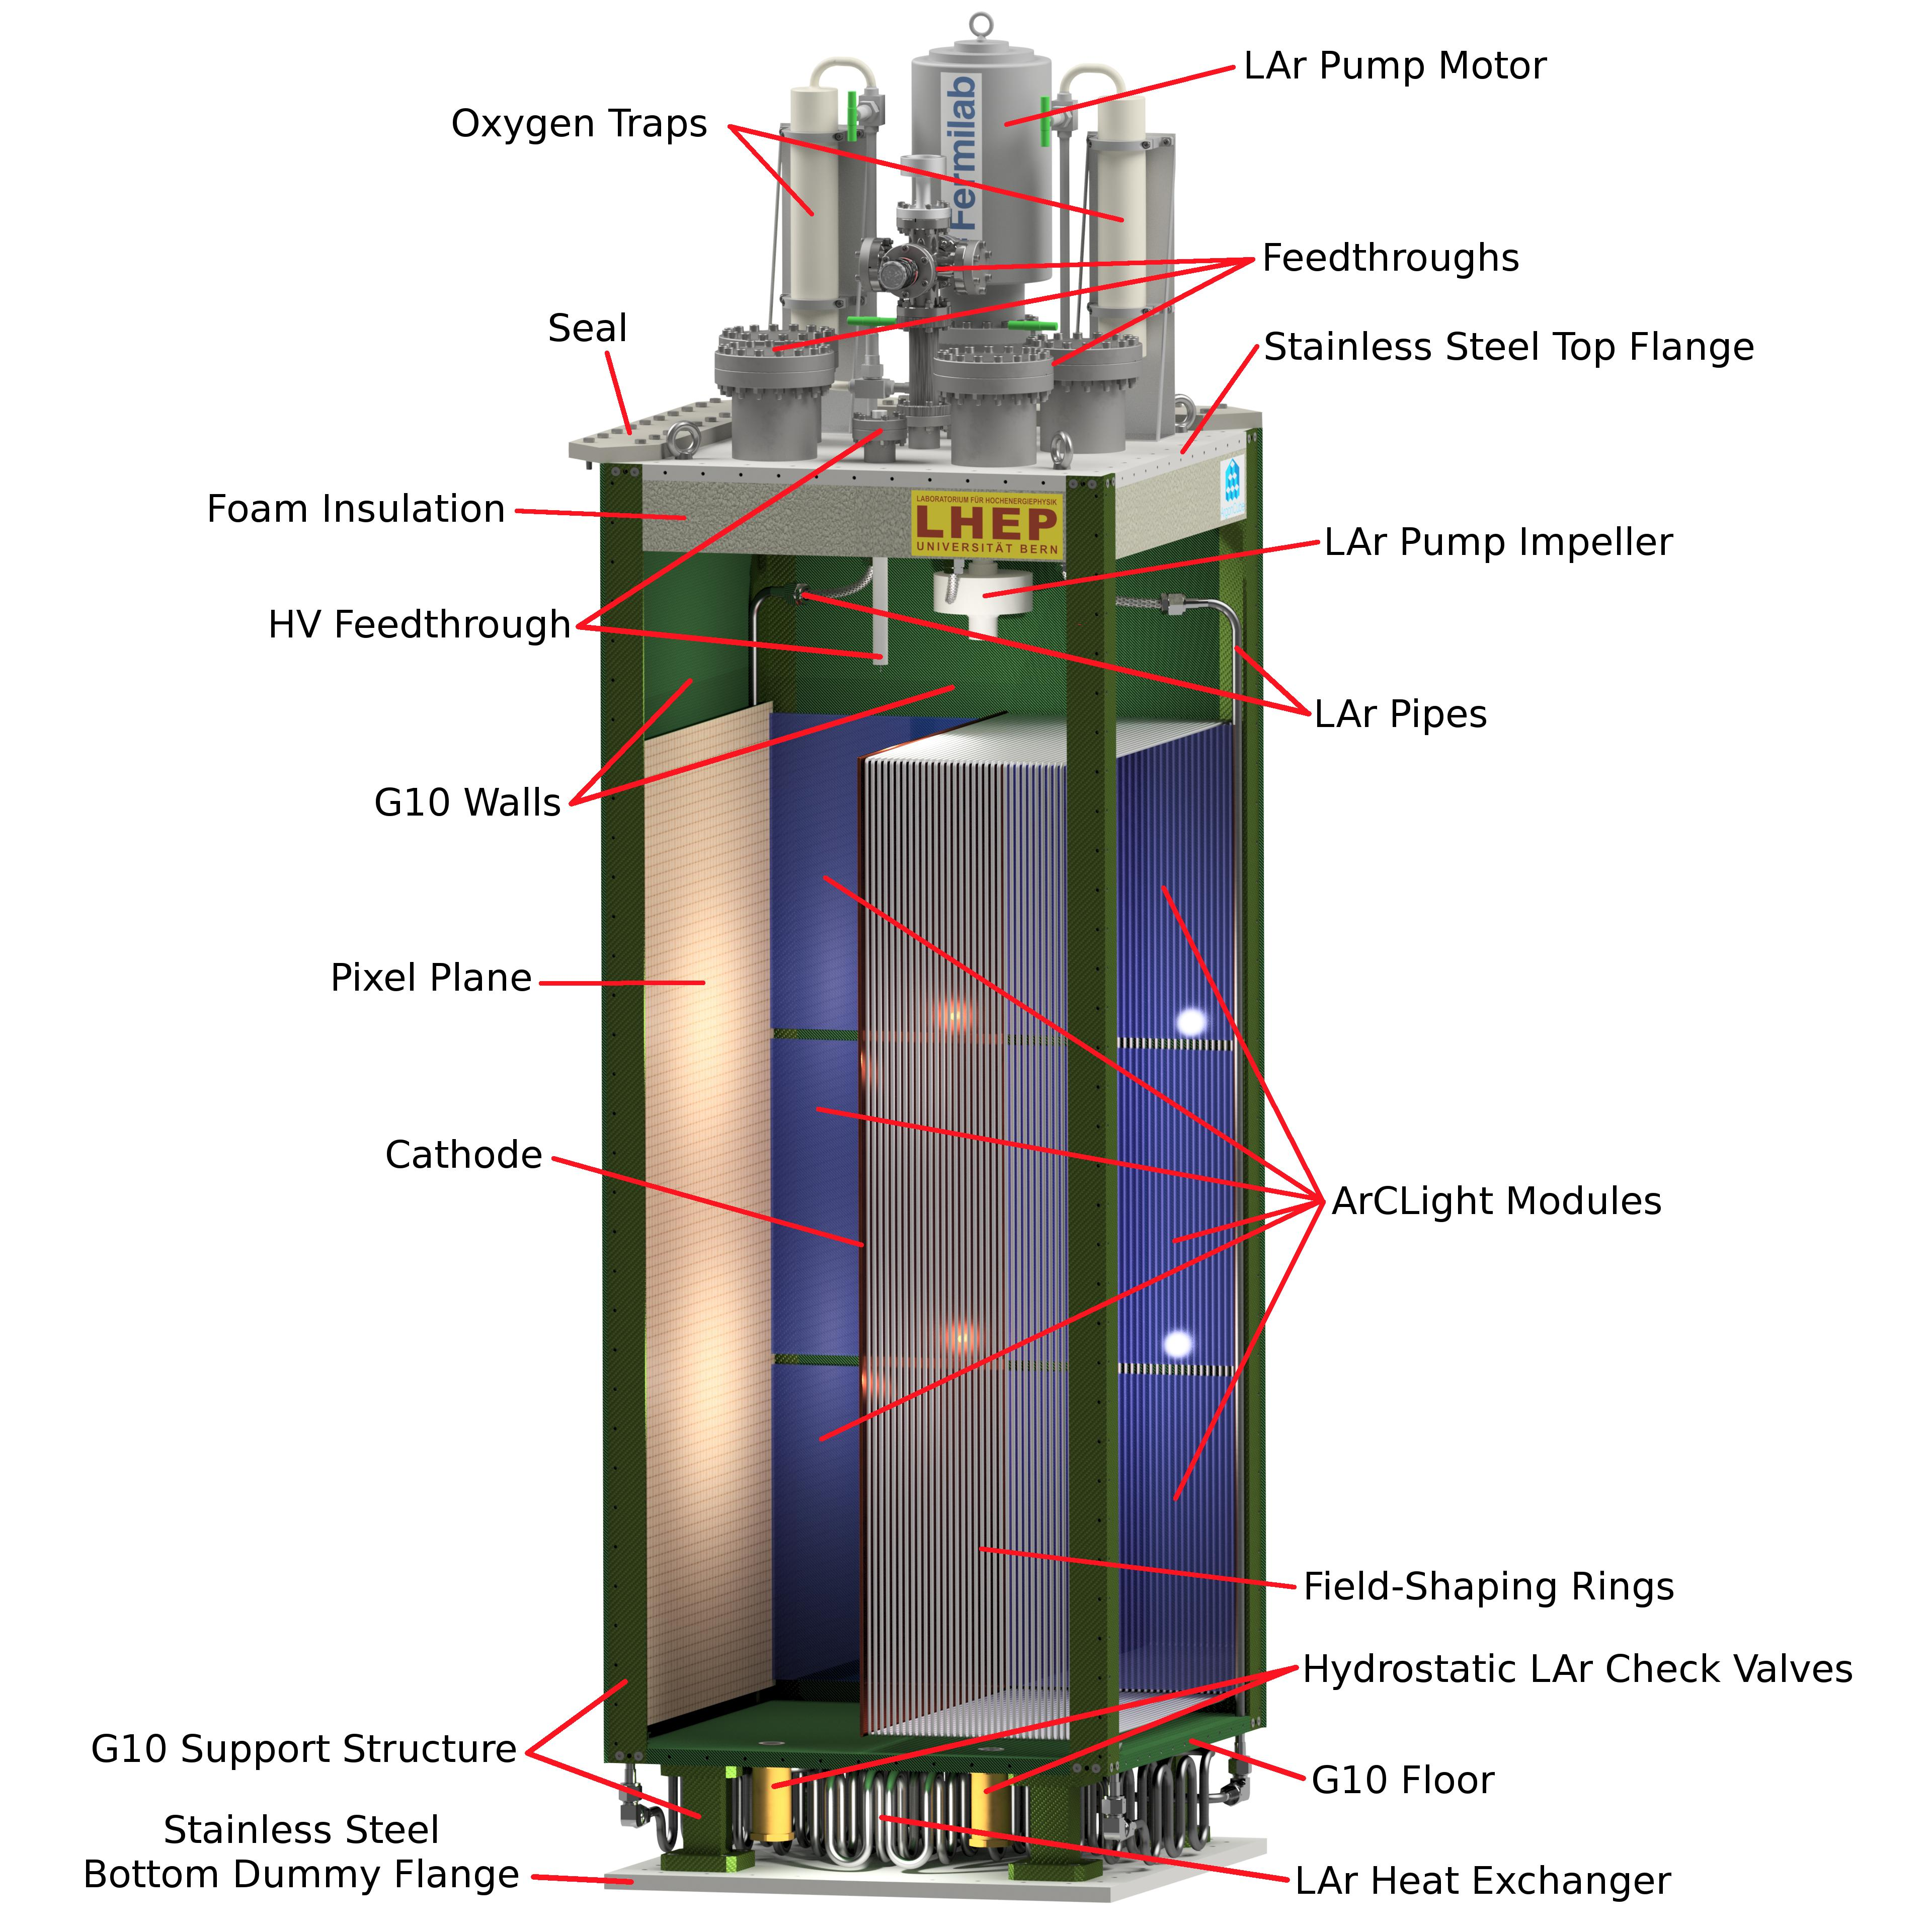
\includegraphics[width=0.8\textwidth]{plots/Normal-Module-4K_labelled.png}
  \caption[ArgonCube module engineering drawing]{Cutaway drawing of a \SI{0.67 x 0.67 x 1.81}{\metre} ArgonCube module for the 2x2 Demonstrator module. For illustrative purposes the drawing shows traditional field shaping rings instead of a resistive field shell. Note, G10 walls will completely seal the module, isolating it from the neighbouring modules and the outer liquid argon bath.}
  \label{fig:ac_module}
\end{figure}

A cutaway drawing of an individual 2x2 module is shown in Figure~\ref{fig:ac_module}. The side walls of each module are made from \SI{1}{\centi\metre} G10 sheets, to which the resistive field shell is laminated. G10's electromagnetic radiation length ($X_{\mathrm{0}} = \SI{19.4}{\centi\metre}$) and hadronic interaction length ($\lambda_{\mathrm{int}} = \SI{53.1}{\centi\metre}$)~\cite{pdg_g10} are both comparable to LAr (14.0~cm and 83.7~cm respectively), making G10 structures in LAr almost transparent for passing particles, allowing for a performance comparable to a monolithic detector. G10 provides a strong dielectric, capable of \SI{200}{\kilo\volt\per\centi\metre} at \SI{1}{\centi\metre} thick~\cite{G10Breakdown}. This dielectric shielding eliminates the need for a clearance volume between the TPCs and the cryostat, while also shielding the TPC from field breakdowns in a neighbouring module. 

The module is split into two TPCs by a central cathode made of an additional resistive layer on a G10 substrate. The segmented drift length does not require a high cathode voltage, and minimizes stored energy. For the 2x2 module footprint of \SI{0.67 x 0.67}{\metre} and an electric field of \SI{1}{\kilo\volt\per\centi\metre} a cathode potential of only \SI{33}{\kilo\volt} is required. The HV is brought into the module using a commercially available feedthrough. Operating a LArTPC at this voltage is challenging, but feasible, without a prohibitive loss of active volume~\cite{argontube}.

The detector is oriented such that the cathodes are parallel to the beam. This minimizes the load on the readout electronics by spreading the event over more channels and reducing the required digitization rate for hit channels. In turn, this reduces the heat load generated at the charge readout and prevents localized boiling.


During module insertion and extraction, the argon flow is controlled by hydrostatic check valves located at the module bottom, which require a minimal differential pressure to open. Purity inside each module is maintained by means of continuous LAr recirculation through oxygen traps. Dirty argon is sucked in at the module top and then pushed through the oxygen traps, clean argon is first routed through a heat exchanger, located below the module inside the outer bath, for cooling and then re-enters the module at the base of the active volume. For optimal heat transport the argon flow is directed along the cold electronics. To prevent dirty argon from the bath entering the modules their interior is held at a slight overpressure, just below the opening pressure of the check valves. For the 2x2 Demonstrator each module will have its own pump and filters, this will not be the case for the ND. In the ND, a more extensive LAr infrastructure will be employed with LAr extracted and filtered in a plant separate to the detector.  

ArgonCube offers true 3D tracking information using the LArPix pixelated charge readout and cryogenic electronics~\cite{larpix}, which are used to amplify and digitize the single-pixel signals in the cold to avoid any analogue multiplexing, and produce unambiguous 3D information. Pixelated anode planes are located on the two module walls parallel to the cathode. The baseline design is for a 5 mm pixel pitch. The LArPix electronics, and a summary of their associated R\&D work, are described in Ref.~\cite{larpix}.

\begin{figure}[!ht]
\centering
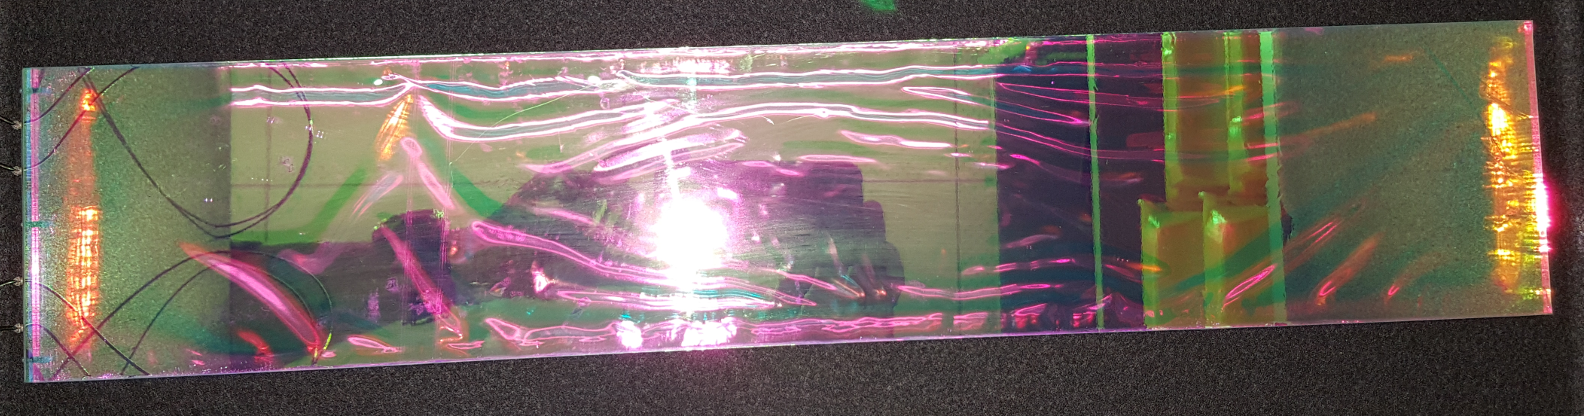
\includegraphics[width=0.75 \linewidth]{plots/1Film50x10.png}
\caption{A prototype ArgonCube light readout paddle built at the University of Bern. The paddle is 50~cm long and 10~cm wide, with four SiPMs coupled to one end. Reproduced from Ref.~\cite{argoncube_loi}.}
\label{fig:arclight}
\end{figure}

With LArPix, the reconstruction issues in a high rate environment are drastically simplified with respect to traditional projective wire readout TPCs. However, the charge readout window (drift time) is \SI{137}{\micro\second} and the beam spill is only \SI{10}{\micro\second}~\cite{numi}, so to correctly reconstruct events overlapping in this window, scintillation signals need to be correctly matched to charge signals (flash matching). If these are correctly matched, the prompt scintillation light defines the time at which ionization electrons start to drift, and the time it takes to register charge on the anode plane along with the electric field strength allow give you enough information to reconstruct the third spatial co-ordinate (along the drift direction). In a modular detector, this problem can easily be simplified using an opaque cathode and module walls, which contains scintillation light in each TPC (half module), and effectively reduce the event pile-up. Furthermore, attenuation due to Rayleigh scattering, $6.6\times10^{-1}$~m~\cite{Rayleigh}, is much less of a problem than in large monolithic detectors given maximum photon propagation lengths of only \SI{0.3}{\metre}. It is desirable to have a large area photon detection system to maximize the utility of scintillation light signals in the detector. However, the downside to modularization is the dead regions between adjacent TPCs, which introduce gaps in the reconstruction, so any light detection system must be compact. The solution pursued for the ArgonCube effort is ArCLight~\cite{arclight}, which is a very compact dielectric light trap that allows for light collection from a large area, inside high electric fields. An example ArCLight sheet is shown in Figure~\ref{fig:arclight}. These sheets are mounted on the walls of the module, inside the field shell, aligned with the drift direction, between the anode and the cathode. The additional dead volume of a few \si{\milli\metre} is similar to the one caused by the charge readout in the perpendicular direction.


\todo{James, can you comment on the 2x2 needs from the external infrastructure point of view?}

\subsection{Downstream tracking detectors}
\label{sec:tracking_detectors}
As well as an ArgonCube-like LAr component, the recommendations from the DUNE Near Detector Concept Study Group~\cite{dune_ndcsg} are for there to be additional, downstream tracking detectors in the DUNE ND to tag and measure the energies of particles which exit the downstream face of the LAr detector, and a magnetized component to identify the sign of muons (and other particles). It would therefore enhance the utility of ProtoDUNE-ND, as an intermediate-scale test of the DUNE ND, to include prototypes for these detectors. It would also enhance any additional possible physics outputs from ProtoDUNE-ND, as many events in the high-energy NuMI ME beamline will not be fully contained in the ArgonCube 2x2 Demonstrator module (examples can be seen in Figures~\ref{fig:argonbox_event_display} and~\ref{fig:leaky_event}). Two downstream tracking options considered  by the DUNE Near Detector Concept Study Group are the Three Dimensional Scintillator Tracker (3DST), and the High-Pressure gaseous argon TPC (HPgTPC).

The 3DST is a fully active plastic scintillator detector made of a large number of optically independent 1x1x1 cm$^{3}$ cubes read out in three orthogonal directions by wavelength shifting fibers~\cite{3dst}. The 3DST is envisioned as an upgrade to the plastic scintillator detectors read out in two dimensions used by T2K~\cite{t2k-fgd,t2k-ingrid}, NOvA~\cite{nova} and MINERvA~\cite{minerva-nim}, which will provide better angular resolution. Unfortunately, after consultation with the 3DST steering group, it was found that a large scale prototype suitable for ProtoDUNE-ND will not be available on the required timescale. If the situation changes, we note the desirability of including such a prototype in the proposed ProtoDUNE-ND effort.

The HPgTPC is a high-pressure argon gas TPC which will operate inside a magnetic field~\cite{dune_ndcsg}. Its purpose is two-fold. Firstly, it acts as a downstream tracker for particles exiting the LAr detector, with a superior dE/dx resolution, and the ability to measure the sign and momentum of particles in the magnetic field. Secondly, it offers a lower threshold, higher resolution argon target detector than the LAr component, which may help constrain certain aspects of the model. The HPgTPC needs to be coupled with a further downstream ECal to detect escaping photons, and to provide fast timing to differentiate tracks from multiple interactions. Although a HPgTPC prototype is not ready at the time of writing this proposal, it is expected that a prototype will be produced during ProtoDUNE-ND operation, so the program should be flexible enough to incorporate a new detector component. A downstream ECal is required for the HPgTPC in order to provide fast timing to differentiate different interactions, and to detect photons which will not convert in the argon gas.

As all potential DUNE ND designs identified in Ref.~\cite{dune_ndcsg} include a fast scintillator component, and a 3DST module will not be available on the timescale of ProtoDUNE-ND, it is desirable to see whether elements of the existing MINERvA detector in the NuMI hall can be re-purposed, as the MINERvA experiment will stop taking data in summer 2019, before ProtoDUNE-ND will get underway. This possibility is discussed separately in Section~\ref{sec:MINERvA}, following discussions with members of MINERvA who have expressed an interest in joining the ProtoDUNE-ND effort.

As it is expected that the ProtoDUNE-ND setup may need to be reconfigured, with the addition of more components over time, and because DUNE-PRISM is now the baseline ND design, it is desirable to include a moveable cryogenic system for the ArgonCube 2x2 Demonstrator in ProtoDUNE-ND, which would allow the future moveable cryogenics for DUNE-PRISM to be tested.

